%%%%%%%%%%%%%%%%%%%%%%%%%%%%%%%%%%%%%%%%%%%%%%%%%%%%%%%%%%%%%%%%%%%%%%%%%%%%%%%	
	\begin{frame}{}
		\begin{bibunit}[abbrv]
			\nocite{Holt1999b}
			\putbib
		\end{bibunit}
	\end{frame}
%%%%%%%%%%%%%%%%%%%%%%%%%%%%%%%%%%%%%%%%%%%%%%%%%%%%%%%%%%%%%%%%%%%%%%%%%%%%%%%%
	\begin{frame}{Plant Model without control}{Tomato Leaf Curl Virus Disease Using an Epidemiological Model}
		\begin{textblock*}{60mm}(65mm,25mm)
			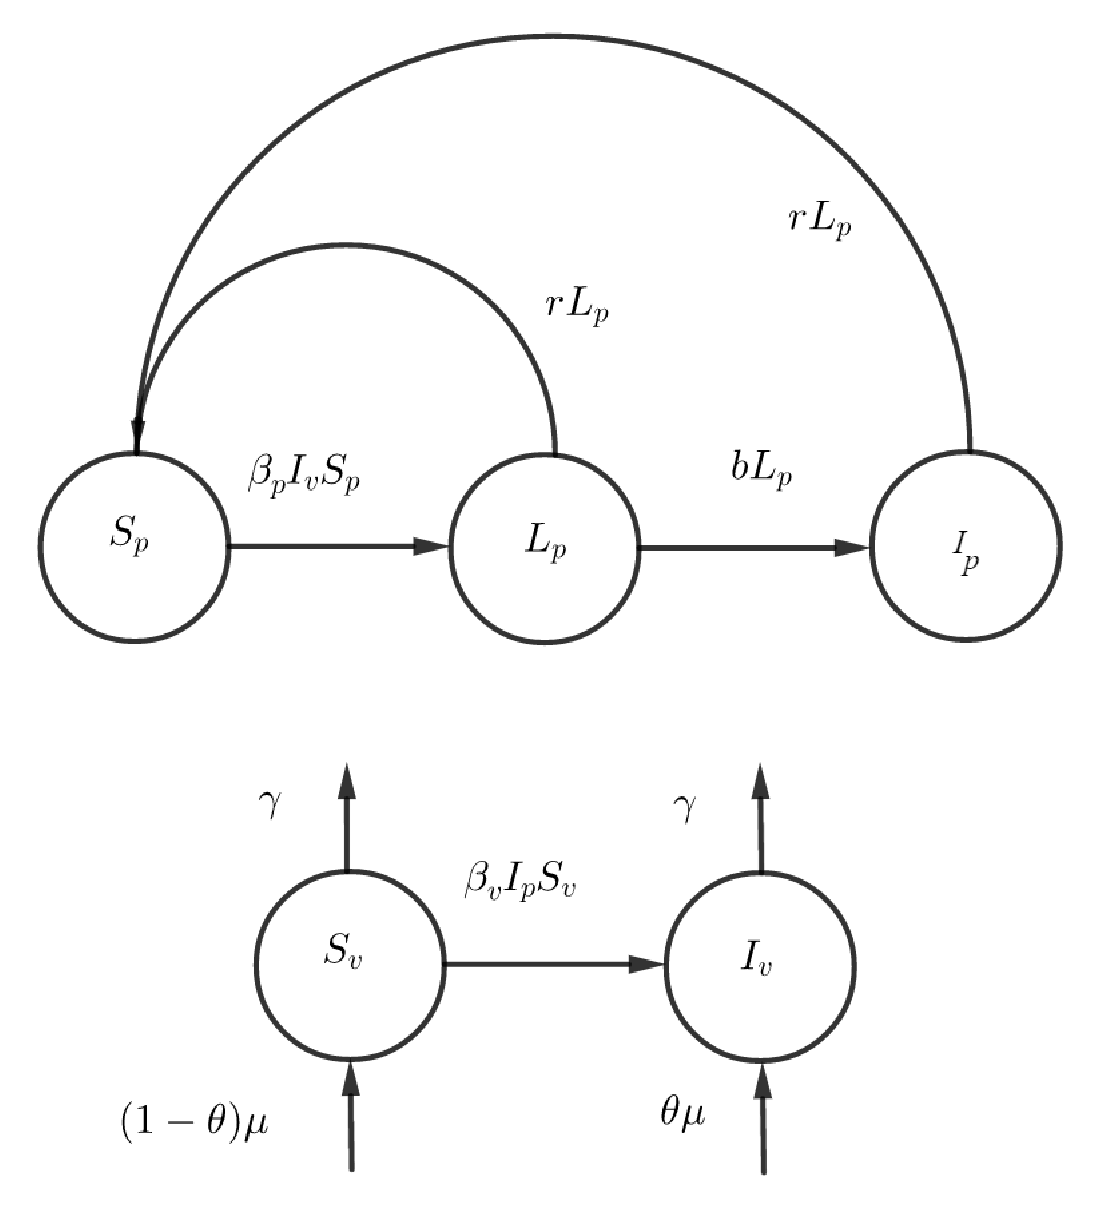
\includegraphics[width=\linewidth]{Feathergraphics/plant_diagram.eps}
		\end{textblock*}
		\begin{textblock*}{55mm}(5mm,25mm)
			\begin{graybox}{Hypothesis:}
				
				\begin{itemize}
					\item infection by infeted plants and vectors,
					\item output and input for plants and vectors. 
				\end{itemize}
			\end{graybox}	
		\end{textblock*}
	\end{frame}
%%%%%%%%%%%%%%%%%%%%%%%%%%%%%%%%%%%%%%%%%%%%%%%%%%%%%%%%%%%%%%%%%%%%%%%%%%%%%%%%
	\begin{frame}
		\frametitle{Others Controls}
		\begin{textblock*}{40mm}(2mm,22mm)
			
			\begin{graybox}{Cultural Control}
				\begin{itemize}
					\item<1-> physical barriers,
					\item<2-> planting dates,
					\item<3-> removal of infested plants,
					\item<4-> host plant resistance.
				\end{itemize}
			\end{graybox}
		\end{textblock*}
		
		\begin{textblock*}{40mm}(43mm,22mm)
			\begin{graybox}{Biological control}
				\begin{itemize}
					\item<5-> Parasitoids,
					\item<6-> predators
					\item<7-> fungi.
				\end{itemize}
			\end{graybox}
		\end{textblock*}
		
		\begin{textblock*}{42mm}(85mm,22mm)
			\begin{graybox}{Insecticide}
				\begin{itemize}
					\item<8-> Pymetrozine,
					\item<9-> flupyradifurone,
					\item<10-> cyazypyr.
				\end{itemize}
			\end{graybox}
		\end{textblock*}
		\only<11>
		{
			\begin{textblock*}{90mm}(45mm,47mm)	
				\begin{bibunit}[abbrv]
					\nocite{Shun-xiang2001}
					\putbib
				\end{bibunit}
			\end{textblock*}

			\begin{textblock*}{120mm}(10mm,70mm)
				
				\begin{bibunit}[abbrv]
					\nocite{Smith2014}
					\putbib
				\end{bibunit}
			\end{textblock*}
		}
	\end{frame}
%%%%%%%%%%%%%%%%%%%%%%%%%%%%%%%%%%%%%%%%%%%%%%%%%%%%%%%%%%%%%%%%%%%%%%%%%%%%%%%
\subsection{Model without control}
	\begin{frame}	
		\begin{textblock*}{62mm}(2mm,15mm)
			\begin{greenbox}{}
				\begin{align*}
				\frac{dS_p}{dt} &=-\beta_p S_p I_v +\textcolor{capri}{r}
				(L_p +  I_p),\\
				\frac{dL_p}{dt} &= \beta_p S_p I_v -b L_p 
				-\textcolor{capri}{r} L_p,\\
				\frac{dI_p}{dt} &= b L_p - \textcolor{capri}{r} I_p,\\
				\frac{dS_v}{dt} &=-\beta_v S_v I_p - \textcolor{cadmiumorange}{\gamma} S_v   -(1-\theta)\mu,\\
				\frac{dI_v}{dt} &=  \beta_v S_v I_p -\textcolor{cadmiumorange}{\gamma} I_v	-\theta\mu,\\
				S_p(0) &= S_{p_0}, L_p(0) = L_{p_0}, I_p(0) = I_{p_0},\\
				S_v(0) &= S_{v_0}, I_v(0) = I_{v_0}.
				\end{align*}
			\end{greenbox}
		\end{textblock*}
		
		\begin{textblock*}{60mm}(65mm,15mm)
			\begin{tabular}{|c |c |l |} 
				\hline
				Par. & Value & Descrip. \\ [0.5ex] 
				\hline
				$\beta_p$ & 0.1 & plant latent rate  \\ 
				\hline
				$r$ & 0.01 & plant remove rate \\
				\hline
				$b$ & 0.075 & plant infectious rate\\
				\hline
				$\gamma$ & 0.06 &  vector die or depar rate \\
				\hline
				$\mu$ & 0.3 & immigration rate \\
				\hline
				$\theta$ & 0.2 & infected vectors arrival \\
				\hline
				$\beta_v$ &0.003 & vector infected rate\\ 
				\hline
			\end{tabular}
		\end{textblock*}
		
		\begin{textblock*}{50mm}(70mm,55mm)
			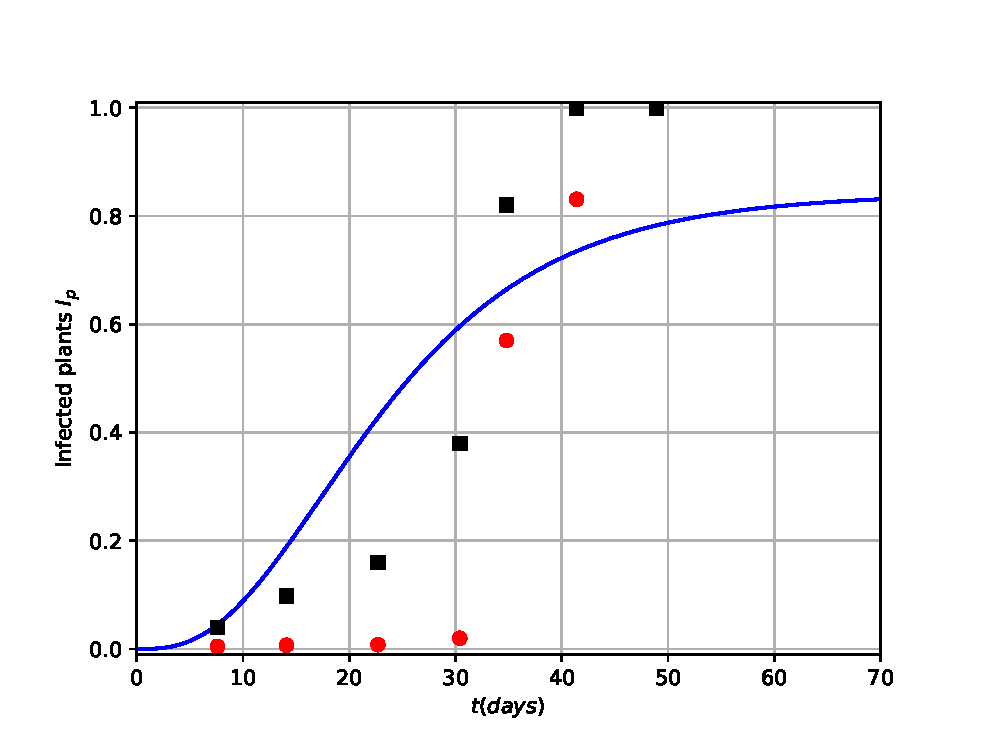
\includegraphics[width=\linewidth]{Feathergraphics/Simulation_data.eps}
		\end{textblock*}
	\end{frame}
%%%%%%%%%%%%%%%%%%%%%%%%%%%%%%%%%%%%%%%%%%%%%%%%%%%%%%%%%%%%%%%%%%%%%%%%%%%%%%%%
	\begin{frame}
		\begin{textblock*}{50mm}(5mm,15mm)
			\begin{greenbox}{}
				\begin{equation*}
				R_0=\sqrt{\frac{\beta_v\mu b\beta_p}{r^2(r+b)\gamma}}.
				\end{equation*}
			\end{greenbox}
			
			\begin{textblock*}{70mm}(5mm,45mm)
				\begin{yellowbox}{}
				\only<1>
				{	
					If $R_0<1,$
					\begin{equation*}
					\lim\limits_{t\rightarrow \infty}(S_p,L_p,I_p,S_v,I_v)=(N_p,0,0,\frac{\mu}{\gamma},0).
					\end{equation*}
				}
				\only<2>
				{
					If $R_0>1,$
					\begin{equation*}
						\lim\limits_{t\rightarrow \infty}(S_p,L_p,I_p,S_v,I_v)=(S_p^*,L_p^*,I_p^*,S_v^*,I_v^*).
					\end{equation*}
				}
				\end{yellowbox}
			\end{textblock*}
			
			
		\end{textblock*}
		\begin{textblock*}{50mm}(77mm,35mm)
			\only<1>
			{
				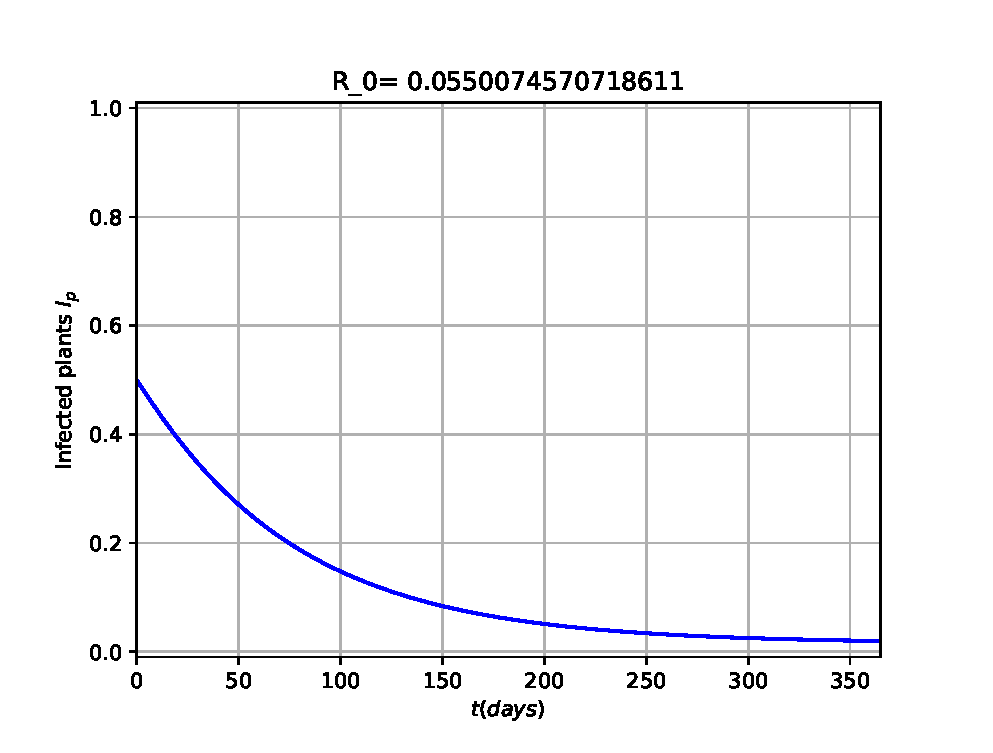
\includegraphics[width=\linewidth]{Feathergraphics/Tomato_simulation_1.eps}
			}
			\only<2>
			{
				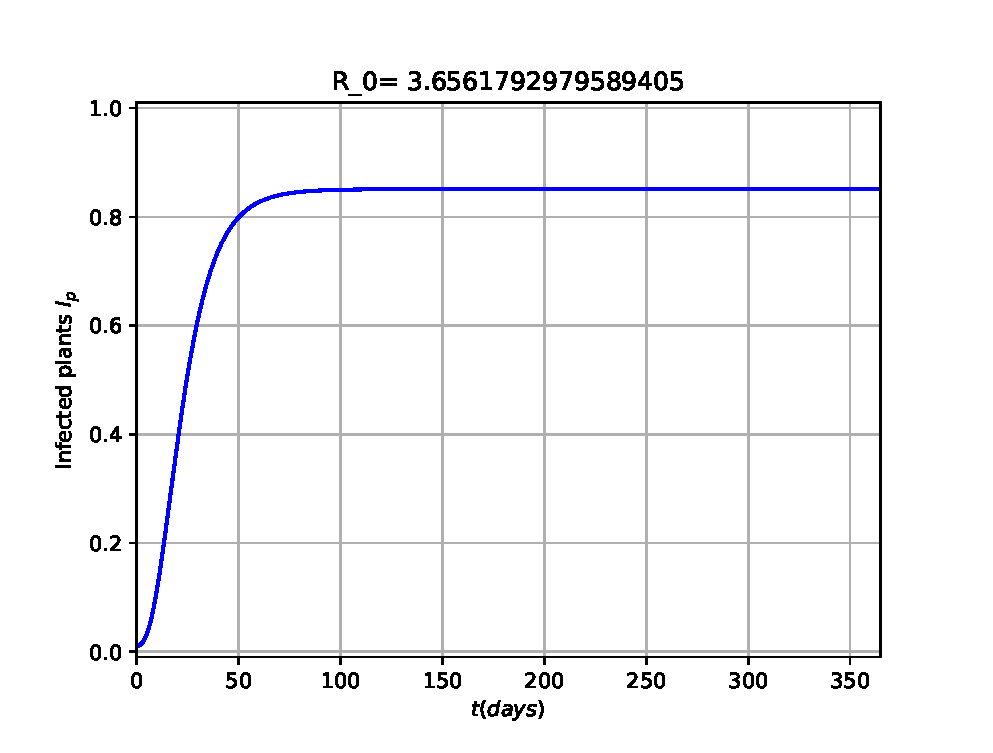
\includegraphics[width=\linewidth]{Feathergraphics/Tomato_simulation_2.eps}
			}
		\end{textblock*}	
	\end{frame}
%%%%%%%%%%%%%%%%%%%%%%%%%%%%%%%%%%%%%%%%%%%%%%%%%%%%%%%%%%%%%%%%%%%%%%%%%%%%%%%%
\subsection{Controlled Model}

	\begin{frame}{Plant Model with control}{Tomato Leaf Curl Virus Disease Using an Epidemiological Model}
		
		\begin{align*}
		\frac{dS_p}{dt} &=-\beta_p S_p I_v +(r +u_1)L_p + (r + u_2) I_p,\\
		\frac{dL_p}{dt} &=\beta_p S_p I_v -b L_p -(r + u_1)L_p,\\
		\frac{dI_p}{dt} &= b L_p - (r + u_2) I_p,\\
		\frac{dS_v}{dt} &=-\beta_v S_v I_p - (\gamma+u_3) S_v -(1-\theta)\mu,\\
		\frac{dI_v}{dt} &=\beta_v S_v I_p -(\gamma+u_3) I_v -\theta\mu,				
		\end{align*}
	\end{frame}
%%%%%%%%%%%%%%%%%%%%%%%%%%%%%%%%%%%%%%%%%%%%%%%%%%%%%%%%%%%%%%%%%%%%%%%%%%%%%%%%
	\begin{frame}
		\begin{textblock*}{120mm}(2mm,12mm)
			Minimize
			\begin{align*}
			J(u_1,u_2,u_3)&=\int_{0}^T	A_1 I_p(t) + A_2 L_p(t) + A_3 I_v(t)
			+ c_1 u_1(t)^2+ c_2 u_2(t)^2\\ &+ c_3 u_3(t)^2 dt,
			\end{align*}
		\end{textblock*}
		\begin{textblock*}{20mm}(2mm,32mm)
			subject to
		\end{textblock*}
		
		\begin{textblock*}{120mm}(20mm,40mm)
			\hspace{50mm}	$\left\{ \begin{array}{ll}
			%				\begin{align*}
			\frac{dS_p}{dt} = &-\beta_p S_p I_v +(r +u_1)L_p + (r + u_2) I_p,\\\\
			\frac{dL_p}{dt} =&\beta_p S_p I_v -b L_p -(r + u_1)L_p,\\\\
			\frac{dI_p}{dt} =& b L_p - (r + u_2) I_p,\\\\
			\frac{dS_v}{dt} =&-\beta_v S_v I_p - (\gamma+u_3) S_v -(1-\theta)\mu,\\\\
			\frac{dI_v}{dt} =&\beta_v S_v I_p -(\gamma+u_3) I_v -\theta\mu,\\\\
			S_p(0) &= S_{p_0}, L_p(0) = L_{p_0},I_p(0) = I_{p_0},S_v(0) = S_{v_0}, I_v(0) = I_{v_0}.			
			%				\end{align*}
			\end{array}\right.$
		\end{textblock*}
	\end{frame}
%%%%%%%%%%%%%%%%%%%%%%%%%%%%%%%%%%%%%%%%%%%%%%%%%%%%%%%%%%%%%%%%%%%%%%%%%%%%%%%%
